In what follows we suppose that we have a function $f(x)$, 
which is continuous and differentiable over the range of interest. 
Let us also assume that we know the value $f(x_0)$ and all the derivatives at $x = x_0$. 

%.......................................
\subsubsection{First order derivatives}

The forward Taylor-series expansion for $f(x_0 + h)$, away 
from the point $x_0$ by a small amount $h$ is given by
\begin{equation}
f(x_0+h)=f(x_0)+ 
h \frac{\partial f}{\partial x}(x_0)  + 
\frac{h^2}{2!} \frac{\partial^2 f}{\partial x^2}(x_0)  +
\dots  +
\frac{h^n}{n!} \frac{\partial^n f}{\partial x^n}(x_0)  
+ {\cal O}(h^{n+1})
\end{equation}
We can substract $f(x_0)$ to each side of the equation and divide by $h$:
\begin{equation}
\frac{1}{h} \left(f(x_0+h)-f(x_0)\right) = 
 \frac{\partial f}{\partial x}(x_0)  + 
\frac{h}{2!} \frac{\partial^2 f}{\partial x^2}(x_0)  + \dots 
\end{equation}
and we can then express the first derivative of $f$ as follows:
\begin{equation}
\frac{\partial f}{\partial x}(x_0) = \frac{f(x_0+h)-f(x_0)}{h} - 
\frac{h}{2!} \frac{\partial^2 f}{\partial x^2}(x_0)  \dots
\end{equation}
or, replacing the term in $h$ by ${\cal O}(h)$:
\begin{equation}
\boxed{
\frac{\partial f}{\partial x}(x_0) = \frac{f(x_0+h)-f(x_0)}{h} + {\cal O}(h)
}
\end{equation}
${\cal O}(h)$ indicates that the full solution would require additional terms of order $h$, $h^2$, 
and so on. ${\cal O}$ is called the {\color{olive}truncation error}: if the distance $h$ 
is made smaller and smaller, the (numerical approximation) error decreases $\propto$ $h$ in this case.

\index{general}{Truncation Error}

Let us assume that the 1D domain on which a given ODE/PDE is to be solved has been discretised
and let us zoom in on three consecutive points:

\begin{center}


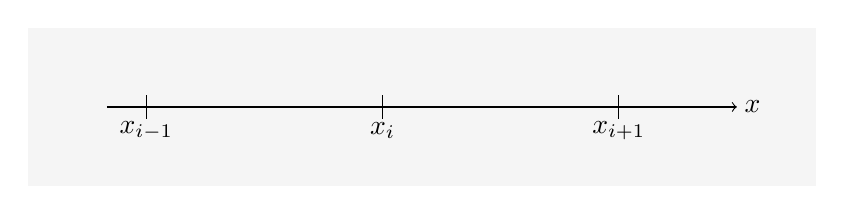
\begin{tikzpicture}
\draw[fill=gray!8,gray!8](0,0) rectangle (10,2);
%\draw[step=0.5cm,gray,very thin] (0,0) grid (8,5); %background grid


%\draw[fill=gray!13,gray!13](1,1) rectangle (8,3);
%\draw[thick] (1,1) -- (5,1) -- (5,4) -- (1,4) -- cycle;  

\draw[->] (1,1) -- (9,1) ; 

\draw[-] (1.5,0.85) -- (1.5,1.15) ; 
\draw[-] (4.5,0.85) -- (4.5,1.15) ; 
\draw[-] (7.5,0.85) -- (7.5,1.15) ; 

\node[] at (1.5,0.7) {$x_{i-1}$};
\node[] at (4.5,0.7) {$x_i$};
\node[] at (7.5,0.7) {$x_{i+1}$};

\node[] at (9.2,1) {$x$};
\end{tikzpicture}

\end{center}

\noindent In the context of a discrete calculation on a set of discrete points $x_i$
we can compute the first order derivative of $f$ at point $x_i$ as an approximation:

\begin{equation}
\boxed{
\frac{\partial f}{\partial x}(x_i) = \frac{f_{i+1}-f_i}{h} + {\cal O}(h) 
}
\qquad
\qquad
\text{(forward difference)} 
\end{equation}
where functions $f_i = f (x_i)$ are evaluated at discretely spaced $x_i$ with $x_{i+1} = x_i + h$ 
(i.e. $h=x_{i+1}-x_i$), where the node spacing, or resolution, $h$ is assumed constant.
We also introduce the notation $f_i'=f'(x_i)=\frac{\partial f}{\partial x} (x_i)$. 


The {\bf forward FD derivative} as expressed above is called {\bf first order accurate},
and this means that very small $h$ is required for an accurate solution.
\index{general}{Forward FD Derivative}
\index{general}{Truncation Error}

%/-/-/-/-/-/-/-/-/-/-/-/-/-/-/-/-/-/-/-/
\begin{center}
\begin{minipage}[t]{0.77\textwidth}
\par\noindent\rule{\textwidth}{0.4pt}
{\color{blue}Example:} Before we go any further with the theory, let us look at a very simple example. 
Let us consider the Stokes equations in the absence of fluid motion (i.e. $\vec\upnu=\vec 0$).
Then the strain rate tensor components are identically zero and the equation simply is 
\begin{equation}
-\vec\nabla p + \rho \vec{g} = \vec 0.
\end{equation}
where we assume that 1) density is constant in space for simplicity and 2)
the domain is infinite in the $x$-direction.
The gravity vector is $\vec{g}=-g \vec{e}_z$ so that the above equation 
becomes:
\begin{equation}
-\frac{dp}{dy} - \rho g = 0
\end{equation}
This is a first-order PDE. It needs to be supplemented by a single boundary condition, 
which in this case constrains the pressure to be zero at the surface, i.e. $p(y=L_y)=0$.


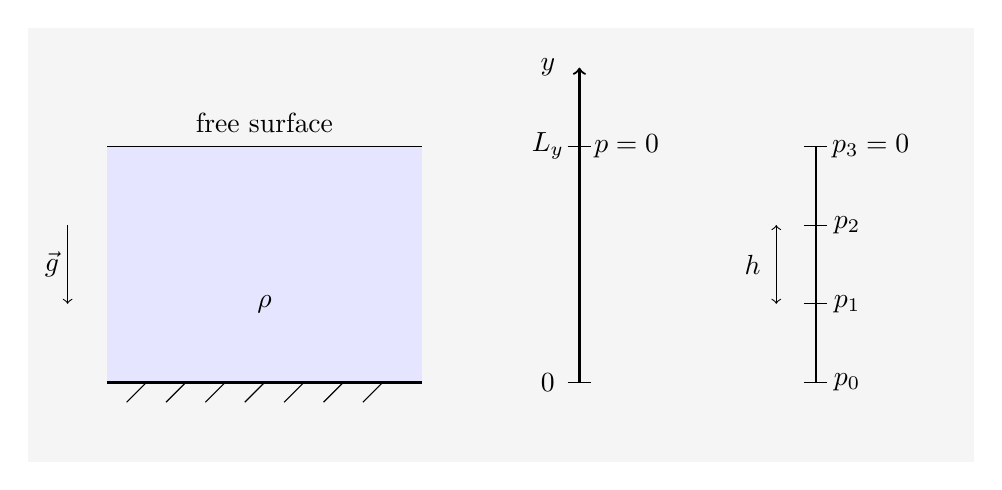
\begin{tikzpicture}
\draw[fill=gray!8,gray!8](0,0) rectangle (12,5.5);
%\draw[step=0.5cm,gray,very thin] (0,0) grid (12,5.5); %background grid

\fill[blue!10!white] (1,1) rectangle (5,4);
\draw[thick,-] (1,1) -- (5,1) ; 
\draw[-] (1,4) -- (5,4) ; 
\draw[->] (0.5,3) -- (0.5,2) ; 
\node[] at (0.3,2.5) {$\vec{g}$};
\node[] at (3,2) {$\rho$};
\node[] at (3,4.3) {free surface};

\draw[-] (1.5,1) -- (1.25,0.75) ; 
\draw[-] (2,1) -- (1.75,0.75) ; 
\draw[-] (2.5,1) -- (2.25,0.75) ; 
\draw[-] (3,1) -- (2.75,0.75) ; 
\draw[-] (3.5,1) -- (3.25,0.75) ; 
\draw[-] (4,1) -- (3.75,0.75) ; 
\draw[-] (4.5,1) -- (4.25,0.75) ; 

%---------------------------------

\draw[thick,->] (7,1) -- (7,5) ; 
\node[] at (6.6,4) {$L_y$};
\node[] at (6.6,1) {$0$};
\draw[-] (6.85,1) -- (7.15,1) ; 
\draw[-] (6.85,4) -- (7.15,4) ; 
\node[] at (7.6,4) {$p=0$};
\node[] at (6.6,5) {$y$};

%---------------------------------

\draw[thick] (10,1) -- (10,4) ; 
\draw[-] (9.85,1) -- (10.15,1) ; 
\draw[-] (9.85,2) -- (10.15,2) ; 
\draw[-] (9.85,3) -- (10.15,3) ; 
\draw[-] (9.85,4) -- (10.15,4) ; 
\node[] at (10.7,4) {$p_3=0$};
\node[] at (10.4,3) {$p_2$};
\node[] at (10.4,2) {$p_1$};
\node[] at (10.4,1) {$p_0$};

\draw[<->] (9.5,2) -- (9.5,3) ;  
\node[] at (9.2,2.5) {$h$};
\end{tikzpicture}




We can write the discretised PDE at node 2 (since we know $p_3=0$):
\begin{equation}
\frac{dp}{dy}(x_2) \simeq \frac{p_3-p_2}{h} = -\rho g
\end{equation}
or, $p_2=\rho g h$. Having obtained $p_2$, we write the PDE at node 1:
\begin{equation}
\frac{dp}{dy}(x_1) \simeq \frac{p_2-p_1}{h} = -\rho g
\end{equation}
or, $p_1= \rho g h + p_2 = \rho g 2h$. And finally we obtain as expected
\begin{equation}
p_0 = \rho g \; 3h = \rho g L_y.
\end{equation}

\par\noindent\rule{\textwidth}{0.4pt}
\end{minipage}
\end{center}

This brings us to our first exercise:

\begin{center}
\begin{minipage}[t]{0.77\textwidth}
\par\noindent\rule{\textwidth}{0.4pt}

\begin{center}

\includegraphics[width=0.8cm]{images/garftr} \\
{\color{orange}Exercise 1}
\end{center}

We will now put the previous example into practice and write a 
python code which uses forward differences to compute the 1D pressure
field inside the crust.

$\rightarrow$ {\tt Exercise\_1\_FDM.ipynb}

\par\noindent\rule{\textwidth}{0.4pt}
\end{minipage}
\end{center}
%/-/-/-/-/-/-/-/-/-/-/-/-/-/-/-/-/-/-/-/







\noindent We can also expand the Taylor series backward (i.e. looking 'left' of $x_0$)
\begin{equation}
f(x_0-h)=f(x_0)-
h \frac{\partial f}{\partial x}(x_0)  + 
\frac{h^2}{2!} \frac{\partial^2 f}{\partial x^2}(x_0)  -
\dots 
\end{equation}
The {\bf backward FD derivative} then writes:
\begin{equation}
\boxed{
\frac{\partial f}{\partial x}(x_i) = \frac{f_{i}-f_{i-1}}{h} + {\cal O}(h) 
}
\qquad
\qquad
\text{(backward difference)} 
\end{equation}

\index{general}{Backward FD Derivative}



Alternatively, we can substract the backward formula from the forward one 
and divide by two. Concretely, we start from 
\begin{equation}
f(x_0+h)=f(x_0)+ 
h \frac{\partial f}{\partial x}(x_0)  + 
\frac{h^2}{2!} \frac{\partial^2 f}{\partial x^2}(x_0)  + \dots  
\end{equation}
and substract the following from it
\begin{equation}
f(x_0-h)=f(x_0)-
h \frac{\partial f}{\partial x}(x_0)  + 
\frac{h^2}{2!} \frac{\partial^2 f}{\partial x^2}(x_0)  + \dots 
\end{equation}
to obtain:
\begin{equation}
f(x_0+h)-f(x_0-h) = 2h \frac{\partial f}{\partial x}(x_0)  +{\cal O}(h^3) 
\end{equation}
or, 
\[
\frac{\partial f}{\partial x}(x_0)  = \frac{ f(x_0+h)-f(x_0-h)}{2h} +{\cal O}(h^2) 
\]
We see that the resulting {\bf central difference} approximation is 
{\bf second order accurate}. In the discrete world one then write
\begin{equation}
\boxed{
\frac{\partial f}{\partial x}(x_i) 
= \frac{f_{i+1}-f_{i-1}}{2h} + {\cal O}(h^2)
}
\qquad
\qquad
\text{(central difference)} 
\end{equation}
Simply put, the denominator is $2h$ because it is the distance between point $x_{i-1}$ and $x_{i+1}$.


\begin{center}
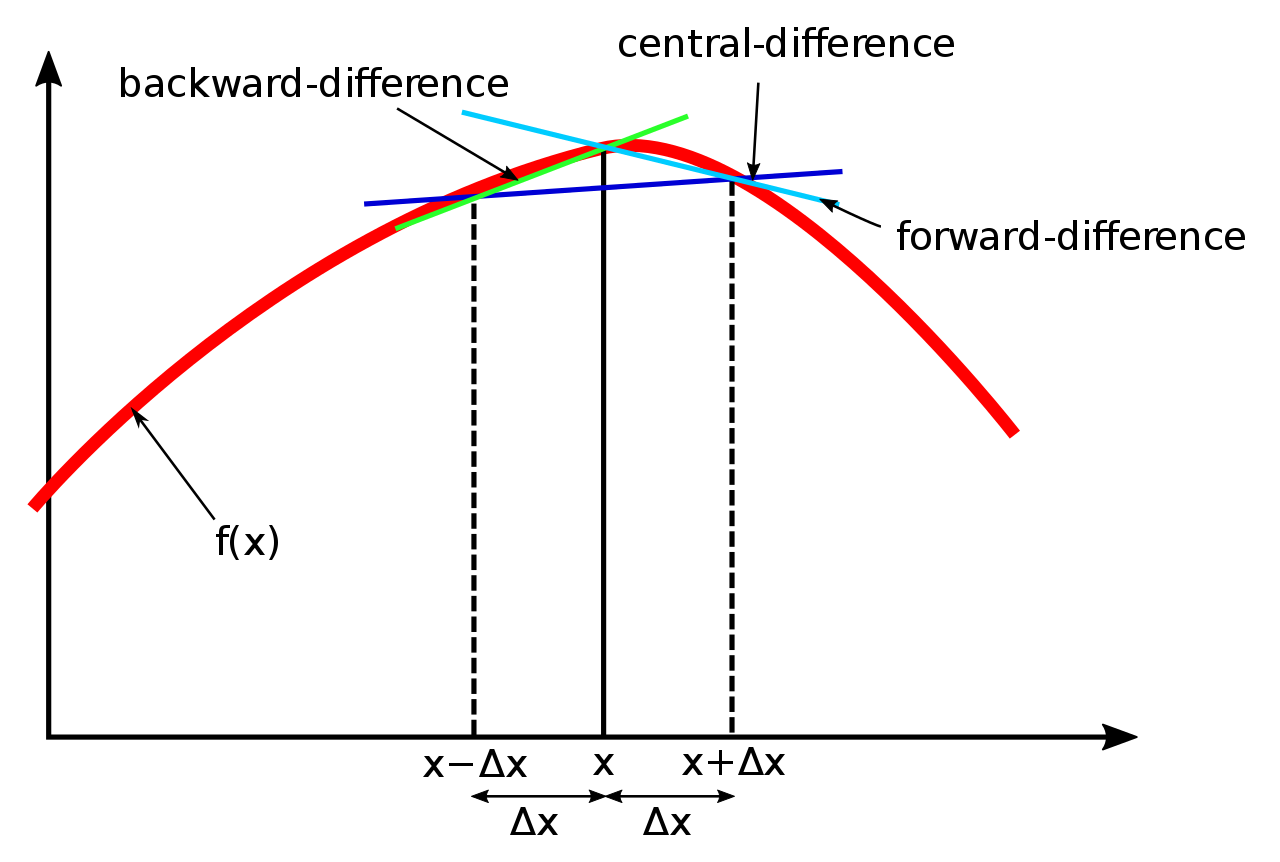
\includegraphics[width=7.7cm]{images/fdm/fd1}\\
{\captionfont 
3 types of the finite difference method. Central gives the best approximation of the derivative.
Taken from Wikipedia\footnote{\url{https://en.wikipedia.org/wiki/Finite_difference}}
}
\end{center}

%.......................................
\subsubsection{Second order derivatives}

Many PDEs contain second order derivatives (typically diffusion equations)
so we now turn to these and 
define $f_i''=f''(x_i) = \frac{\partial^2 f}{\partial x^2} (x_i)$. 

%______________________________
\paragraph{Second order forward} 
Let us define a function $g(x)$ such that $g=f'$. Then we have seen that the forward 
difference formula leads to write: 
\begin{equation}
g_i' = \frac{g_{i+1}-g_{i}}{h}
\end{equation}
On the one hand, we have $g_i'=g'(x_i)=f''(x_i)=f_i''$ and on the other hand
\begin{equation}
\frac{g_{i+1}-g_{i}}{h} = \frac{f_{i+1}'-f_{i}'}{h}
\end{equation}
We can then use the forward derivative formula for $f_{i+1}'$ and $f_{i}'$ and 
obtain the following second order derivatives of $f$:
\begin{equation}
f_{i}'' 
= \frac{f_{i+1}'-f_i'}{h} 
%+ {\cal O}(h^2)
= \frac{\frac{f_{i+2}-f_{i+1}}{h}-
\frac{f_{i+1}-f_i}{h}
}{h} 
%+ {\cal O}(h^2)
= \frac{f_{i+2}-2f_{i+1}+f_i}{h^2} 
%+ {\cal O}(h^2)
\end{equation}
which is the {\bf first order accurate}, {\bf forward difference} approximation for
second order derivatives at $x_{i}$.
In order to compute $f''(x_i)$ we need the value of $f$ at $x_i$ but also at two 
other locations right of this location.

%______________________________
\paragraph{Second order backward}
Likewise, we obtain the following formula when using the backward derivative twice:

\begin{equation}
f_{i}'' 
= \frac{f_{i}'-f_{i-1}'}{h} 
%+ {\cal O}(h^2)
= \frac{\frac{f_{i}-f_{i-1}}{h}- \frac{f_{i-2}-f_{i-1}}{h}  }{h} 
%+ {\cal O}(h^2)
= \frac{f_{i}-2f_{i-1}+f_{i-2}}{h^2} 
%+ {\cal O}(h^2)
\end{equation}
This time we  we need the value of $f$ at $x_i$ but also at two 
other locations left of this location.

%______________________________
\paragraph{Second order central} 
By adding the taylor expansions (with $+h$ and $-h$) 
a {\bf second order accurate}  approximation of the second derivative is obtained.
We start from 

\begin{eqnarray}
f(x_0+h)&=&f(x_0)+ 
h \frac{\partial f}{\partial x}(x_0)  + 
\frac{h^2}{2!} \frac{\partial^2 f}{\partial x^2}(x_0)  +
\dots  +
\frac{h^n}{n!} \frac{\partial^n f}{\partial x^n}(x_0)  
+ {\cal O}(h^{n+1}) 
\\
f(x_0-h)&=&f(x_0) 
-h \frac{\partial f}{\partial x}(x_0)  + 
\frac{h^2}{2!} \frac{\partial^2 f}{\partial x^2}(x_0)  +
\dots  +
\frac{(-h)^n}{n!} \frac{\partial^n f}{\partial x^n}(x_0)  
+ {\cal O}(h^{n+1}) 
\end{eqnarray}
and we see that adding the first equation to the second yields
\begin{equation}
f(x_0+h) + f(x_0-h) =2 f(x_0)+ 
\underbrace{h \frac{\partial f}{\partial x}(x_0)   
-h \frac{\partial f}{\partial x}(x_0)}_{=0}  + 
\frac{h^2}{2!} \frac{\partial^2 f}{\partial x^2}(x_0)  +
\frac{h^2}{2!} \frac{\partial^2 f}{\partial x^2}(x_0)  
+ {\cal O}(h^{3})
\end{equation}
or, 
\begin{equation}
\frac{\partial^2 f}{\partial x^2}(x_0)  =
\frac{f(x_0+h) -2f(x_0) + f(x_0-h) }{h^2}
+ {\cal O}(h)
\end{equation}
which translates into
\begin{equation}
\boxed{
f_{i}''=\frac{f_{i+1}-2f_i+f_{i-1}}{h^2} + {\cal O}(h)
}
\qquad
\qquad
\text{(second order central difference)}
\end{equation}
Note that this formula requires one value left and one value right of the point 
under consideration. 

Another way to arrive at the same expression is to write the expansion at $x_0 \pm h/2$, 
i.e. at the (convenient, yet inexistant) half points $i\pm 1/2$:

\begin{center}


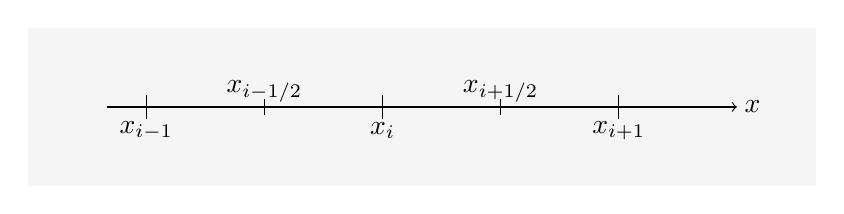
\begin{tikzpicture}
\draw[fill=gray!8,gray!8](0,0) rectangle (10,2);
%\draw[step=0.5cm,gray,very thin] (0,0) grid (8,5); %background grid


%\draw[fill=gray!13,gray!13](1,1) rectangle (8,3);
%\draw[thick] (1,1) -- (5,1) -- (5,4) -- (1,4) -- cycle;  

\draw[->] (1,1) -- (9,1) ; 

\draw[-] (1.5,0.85) -- (1.5,1.15) ; 
\draw[-] (4.5,0.85) -- (4.5,1.15) ; 
\draw[-] (7.5,0.85) -- (7.5,1.15) ; 

\node[] at (1.5,0.7) {$x_{i-1}$};
\node[] at (4.5,0.7) {$x_i$};
\node[] at (7.5,0.7) {$x_{i+1}$};

\node[] at (3,1.2) {$x_{i-1/2}$};
\node[] at (6,1.2) {$x_{i+1/2}$};
\draw[-] (3,0.9) -- (3,1.1) ; 
\draw[-] (6,0.9) -- (6,1.1) ; 

\node[] at (9.2,1) {$x$};
\end{tikzpicture}

\end{center}


%\begin{verbatim}
%     
%                              x_{i-1/2)           x_{i+1/2}
%               --------|----------+----------|---------+----------|-------------> x
%                     x_{i-1}                x_i                x_{i+1}
%
%\end{verbatim}

\begin{equation}
f_{i+1/2}'=\frac{f_{i+1}-f_i}{h}
\quad\quad
\quad\quad
f_{i-1/2}'=\frac{f_{i}-f_{i-1}}{h}
\end{equation}
\begin{equation}
f_i''=\frac{f_{i+1/2}'-f_{i-1/2}'}{h} = 
\frac{f_{i+1}-2f_i+f_{i-1}}{h^2} 
\end{equation}

Note that derivatives of the form (see heat transport equation in Section~\ref{ss:hte}) 
\begin{equation}
\frac{\partial }{\partial x} \left(  k  \frac{\partial f}{\partial x} \right)
\end{equation}
where $k$ is a function of space, should be formed as follows
\begin{equation}
\left. \frac{\partial }{\partial x} \left(  k  \frac{\partial f}{\partial x} \right) \right|_i
=
\frac{ k_{i+1/2} \frac{f_{i+1}-f_i}{h} - k_{i-1/2}\frac{f_i-f_{i-1}}{h}    }{h} + {\cal O}(h^3)
\end{equation}
where $k_{i\pm 1/2}$ is evaluated between the points to maintain the second order accuracy.

\begin{remark}
If the heat conductivity $k$ shows strong jumps from one grid point to another that are not aligned with
the grid-nodes, most second-order methods will show first order accuracy at best.
\end{remark}






